\chapter{Network Design}

\section{Topology}

The topology used for this lab assignment takes form as a three router set-up,
this simulates the infrastructure that a typical Internet Service Provider may
have. Using three routers as opposed to a single router allows for the ISP to
include additional technologies such as dynamic internal routing and iBGP in
order to create a fault-tolerant network. With multiple devices used in the
Service Provider topology the network will have increased uptime as traffic can
be routed via an alternate path should any outage occur on a single device.

\begin{figure}[!ht]
	\caption{High-level Topology}
	\centering
	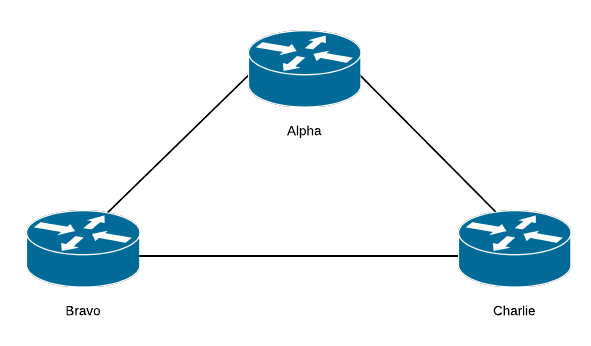
\includegraphics[width=0.8\textwidth]{images/networkTopology.png}
\end{figure}

The topology used for this lab assignment takes form as a three router set-up,
this simulates the infrastructure that a typical Internet Service Provider may
have. Using three routers as opposed to a single router allows for the ISP to
include additional technologies such as dynamic internal routing and iBGP in
order to create a fault-tolerant network. With multiple devices used in the
Service Provider topology the network will have increased uptime as traffic can
be routed via an alternate path should any outage occur on a single device.

\section{Address Allocation}
\subsection{IPv4}
For this lab exercise we were assigned the IP block 12.0.0.0/8 for our ISP, BT.
As this address space provides BT with 16.7 million addresses to allocate it was
easy to be naive with the allocation to subnets in our internal network.
However, taking into account the issues that arose from the original allocation
of IPv4 network blocks to ISPs and Educational Institutions it was decided that
wasting address space by using unnecessarily small subnet masks should be
avoided. Within our IPv4 topology we have three classifications of addresses
used; Customer segments, Point-to-point links and Loopback addresses. The
classification of these network types are outlined in
Figure~\ref{figure:network-alloc-1}.

\begin{figure}[!ht]
	\caption{Network Allocations}
	\label{figure:network-alloc-1}
	\centering
	\begin{tabular}{|c|c|p{5.5cm}|}
		\hline \textbf{Address Type} & \textbf{Subnet Mask} & \textbf{Justification} \\
		\hline Customer Segment & /24 & These segments are allocated to downstream customers, at current these are allocated enough address space for 254 devices. In our network Laptops are used on these segments to test connectivity to customers. The size of this subnet also allows for easy identification of subnets to their location in the topology  \\
		\hline Point-to-point Links & /30 & This specification is used for links that connect two routers, for these links only two IP Addresses are required and a /30 subnet mask is the smallest mask that will provide this. \\
		\hline Loopback Address & /32 & Addresses used for the loopback interfaces on the routers, there is only a requirement for a single address and a /32 mask produces this \\
		\hline
	\end{tabular}
\end{figure}

In addition to the allocation of subnets based on size, the ISP also uses the
addresses encompassed in the block as an identifier for it's location in the
network. Using the value of a particular octet in a network address was a schema
that was created in advance of the network build-out and allowed for easy
identification of issues in IP or interior routing configurations. These schemas
are outlined in Figure~\ref{figure:network-alloc-2}.

\begin{figure}[!ht]
	\caption{Network Allocations}
	\label{figure:network-alloc-2}
	\centering
	\begin{tabular}{|c|p{8cm}|}
		\hline \textbf{Address Allocation} & \textbf{Identifying Feature} \\
		\hline 12.0.\#.0/24 & The hash in this address dictates the router that this address space is connected to, with 1 corresponding to Alpha etc. This would scale for up to 253 subnets in the Service Provider \\
		\hline 12.\#.0.0/24 (10+) & The hash in these networks dictate the assigned number of the group we connect to on these links. This enables us to quickly identify the group involved with any connectivity issues in BGP  \\
		\hline 12.\#.\#.\# & This schema was used for loopback addresses on the routers, the hash is the same value in all three octets of the address and dictates the router that this loopback is assigned to. For example, 12.3.3.3/32 is the loopback address of Charlie \\
		\hline
	\end{tabular}
\end{figure}
\clearpage

\subsection{IPv6}